\section{Существующие проблемы разработки языков программирования}
Создание трансляторов для языков программирования вообще, и проблемно"=ориентированных языков в частности, с помощью распространенных сегодня техник \cite{redDragon,hanter} --- задача крайне трудоемкая. Кроме того, в последние годы, благодаря усилиям компании "<JetBrains">, требования к средам разработки существенно возросли. Мартин Фаулер даже ввел термин "<post-Intellij world"> \cite{fowler01}, означающий мир после создания компанией "<JetBrains"> среды разработки "<IntelliJ IDEA"> \cite{intellijIDEA}, качественно изменивший представление о возможностях сред разработки. То есть в настоящее время, создания транслятора недостаточно для того, чтобы языком можно было пользоваться также эффективно, как языками общего назначения, для которых существуют развитые среды разработки. Это не позволяет создавать узкоспециализированные проблемно-ориентированные языки, которые были бы очень эффективны для решения небольшого класса задач, но выгода от использования таких языков нивелируется затратами на их разработку.

В связи с этим в компании "<JetBrains"> была разработана среда для создания и использования проблемно-ориентированных языков программирования \MPS{} \cite{dmitriev,fowler02}. Эта среда позволяет существенно упростить процесс создания языков программирования, средств для программирования на них и интеграции с существующими технологиями и языками.

По мнению разработчиков среды \MPS{}, способ хранения исходного кода программы в виде набора текстовых файлов, накладывает серьезные ограничения на возможности языка программирования и неоправданно усложняет процесс трансляции. Каждый раз при компиляции необходимо строить абстрактный семантический граф (АСГ) \cite{portableSourceCode} программы, состоящий из абстрактных синтаксических деревьев (АСД) \cite{plopAST} для модулей программы и таблиц ссылок между узлами этих деревьев. В тоже время, для построения подсказок при вводе (autocompletion) \cite{myAutocompletion}, подсветки ошибок в коде, автоматических рефакторингов \cite{fowler03} и других действий характерных для  интеллектуальных сред разработки, также необходим АСГ программы. Поэтому целесообразно хранить исходный код программы непосредственно в виде АСГ \cite{simonyi}. Такой подход весьма распространен для графических языков программирования \cite{myUMLSwitchEclipse,gmf,msdsl}.

Вместе с тем, уже существуют эффективные способы автоматизации редактирования формальных текстов и навигации по ним. Большинству программистов текстовое представление наиболее привычно. Этим объясняется не слишком широкое распространение графических проблемно-ориентированных языков. Учитывая это, редакторы АСГ в среде MPS реализованы так, чтобы быть максимально похожими на обычные текстовые редакторы интеллектуальных сред разработки \pic{\ref{fig:ClassInMPS}}.

\begin{figure}
\centering
\fbox{
 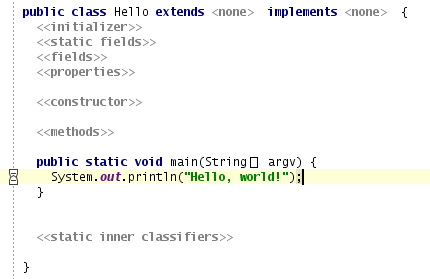
\includegraphics[width=0.9\textwidth]{ClassInMPS.png}
}
\caption{Редактор для класса в среде \MPS{}}
\label{fig:ClassInMPS}
\end{figure}
